\chapter{Results}\label{chapter:results}
Following providing the multivariate analysis technique described in Section~\ref{sec:mvas} with the simulated samples, and their systematic variations, and data, the resultant set of BDT discriminator distributions can be used to perform a measurement.

The following chapter describes the statistical methodology used to analyse these distributions and produce the first measurement of the signal process' cross section along with its expected significance.
Following a discussion of the impact that the systematic uncertainties have on the fitted results, the result presented is compared with those from the already published searches for tZq production made using the trilepton final state.

\section{Statistical Methodology}\label{sec:statisticalModel}
The Higgs Analysis Combined Limit (\combine) tool~\cite{Combine} tool, a framework based on the RooStats package~\cite{Moneta:2010pm,Schott:2012zb}, was used to perform a binned Maximum Likelihood Fit (MLF) to analyse the measurement made using the $CL_{S}$ method~\cite{CMS-NOTE-2011-005,Khachatryan:2014jba,AsymptoticFormulae}.

\subsection{Likelihood Model}\label{subsec:likelihoodModel}
For the signal and background processes considered in the search, the expected event yield $\lambda$ in bin $i$ of the distribution considered (\ie the BDT discriminator) is given by Equation~(\ref{eq:yields1}):

\begin{equation}
\lambda_{i} = \mu s_{i} + \sum\limits_{j}^{n_{bkgs}} b_{j} \;
\label{eq:yields1}
\end{equation}

where $s$ and $b$ are the expected number of signal and background events, respectively, the index $j$ runs over the number of background sources, $n_{bkgs}$, and $\mu$ is the signal strength modifier.
The signal strength modifier is typically used instead of directly determining the expected (and observed) cross section of a process as it makes the comparison of different results (particularly from different experiments) more straightforward. 
The relationship between $\mu$ and the observed and expected cross sections, $\sigma_{obs}$ and $\sigma_{s}$, is given by Equation(~\ref{eq:signalModifier}):

\begin{equation}
\mu = \frac{\sigma_{obs}}{\sigma_{s}}  \;
\label{eq:signalModifier}
\end{equation}
 
The uncertainties associated with the simulated predictions for the signal and background processes are accounted for by the inclusion of a set of nuisance parameters $\theta$.
Therefore, as $s_{i}$ and $b_{i}$ are dependent on $\theta$, they become $s_{i} = s_{i} (\theta)$ and $b_{i} = b_{i} (\theta)$.

Assuming that the number of observed events, $n_{i}$, in any given bin of the distribution considered will be distributed according to Poisson statistics, the probability of observing $n_{i}$ is given by Equation~(\ref{eq:poissonProb}):

\begin{equation}
\mathcal{P} ( n_{i} | \lambda_{i} ) = \frac{\lambda_{i}}{n_{i}!} e^{- \lambda_{i}} = \frac{ \big( \mu s_{i}(\theta) + b_{i}(\theta) \big)^{n_{i}}}{n_{i} !} e^{- \mu s_{i}(\theta) - b_{i}(\theta)}  \;
\label{eq:poissonProb}
\end{equation}

A probability density function, $\rho ( \theta | \tilde{\theta} )$ is used to describe all the sources of uncertainty for the nuisance parameters, where $\tilde{\theta}$ is the set of nominal values for the the best estimate of the nuisances.
For the search presented in this thesis, it is assumed that each source of systematic uncertainty is either 100\% correlated or uncorrelated.
This allows each systematic uncertainty to be incorporated into the likelihood function in a clean factorised form.
Shape uncertainties are modelled by vertically morphing the nominal shape template up and down by one $\sigma$.
The normalisation/rate uncertainties are treated as log-normal distributed nuisance parameters~\cite{Baak:2014fta,AsymptoticFormulae}.
%%% log-uniform - for NPL to allow it to be simultaneously fitted with the signal normalisation

Thus, the likelihood for the entire dataset can be expressed as the product of the Poisson probabilities, $\mathcal{P}$, for all bins and the nuisance parameters' probability density function, as given by Equation~(\ref{eq:poissonLikelihood}).

\begin{equation}
\mathcal{L} ( n_{i} | \mu , \theta ) = 
\prod_{i=1}^{N} \mathcal{P} \big( n_{i} | \mu s_{i}(\theta) + b_{i}(\theta) \big) \rho ( \theta | \tilde{\theta} ) \;
\label{eq:poissonLikelihood}
\end{equation}

\subsection{$CL_{S}$ method}\label{subsec:CLsMethod}
The modified classical frequentist method, known as the $CL_{S}$ method, was used to evaluate the compatibility of data with the \emph{signal plus background} (s+b) and \emph{background only} (b-only) hypotheses in terms of the signifiance of, and the limits on, the measured signal strength ~\cite{AsymptoticFormulae}.

To evaluate these hypotheses, the $CL_{S}$ method constructs a test statistic, $q_{\mu}$.
The test statistic used by the ATLAS and CMS is defined as the loglikelihood ratio in equation~\ref{eq:testStatistic},

\begin{equation}
q_{\mu} =  -2 \ln \frac{ \mathcal{L}(data | \mu s , \hat{\theta_{\mu}})} { \mathcal{L}(data | \hat{\mu} s \hat{\theta_{\mu})  }} \textrm{ , where } 0 \leq \hat{\mu} \leq \mu \;
\label{eq:testStatistic}
\end{equation}

where $\hat{\theta_{\mu}}$ refers to the maximum likelihood estimators of $\theta$ for a given $\mu$, and 
$\hat{\mu}$ and $\hat{\theta}$ correspond to the global maximum of the likelihood. 
By definition $\hat{\mu}$ cannot take negative values as physics defines the signal rate as positive. 
The constraint $\hat{\mu} < \mu$ is applied to ensure a one-sided confidence interval.

As the analysis was initially conducted blind, \emph{pseudo-data} was generated for the \emph{expected} outcomes in order to construct probability distribution functions for the s+b and b-only hypotheses for a given signal strength.
For the unblinding of the analysis, the \emph{observed} measurement was made by replacing the pseudo-data used for the s+b probability distribution functions with the actual data.
From these probability distribution functions, the probability values for the s+b and b-only hypotheses can be defined as Equations~(\ref{eq:pmu})-(~\ref{eq:1-pb}):

\begin{equation}
p_{\mu} = P ( q_{\mu} \geq  q_{\mu}^{obs} | \mu s + b ) = \int^{\infty}_{q_{\mu}^{obs}} f ( q_{\mu} | \mu , \theta_{\mu}^{obs} ) dq_{\mu} \;
\label{eq:pmu}
\end{equation}

\begin{equation}
1 - p_{b} = P ( q_{\mu} \geq  q_{\mu}^{obs} | b ) = \int^{\infty}_{q_{0}^{obs}} f ( q_{\mu} | 0 , \theta_{0}^{obs} ) dq_{\mu} \;
\label{eq:1-pb}
\end{equation}

The ratio of these probabilities is used to define $CL_{S} (\mu)$ in Equation~(\ref{eq:CLs}).

\begin{equation}
CL_{S} (\mu) = \frac{ p_{\mu} }{ 1 - p_{b} }\;
\label{eq:CLs}
\end{equation}

If, for a given $\mu$, $CL_{S} < \alpha$, then it is said that the signal process in question is excluded with a $(1 - \alpha)$ Confidence Level (CL).
Therefore, as the 95\% CL upper limit is used in this search, the limit is determined by altering $\mu$  until $CL_{S} = 0.05$.

%\subsection{Asymptotic CL$_{s}$ method}\label{subsec:asymptoticCLS}
Instead of using an ensemble of toy MC samples to generate the pseudo-data, one representative dataset, known as the \emph{Asimov dataset}, was used.
This method, known as the \emph{asymptotic} CL$_{s}$ method, is used when the number of expected events is sufficiently large as it typically reduces the amount of computing time required.
The Asimov dataset is defined as being constructed such that all observable quantities are equal to their expectation values.
A full description of the asymptotic approximation to the CL$_{s}$ method is given in~\cite{AsymptoticFormulae}.

\clearpage
\newpage

\section{Statistical Analysis Results}\label{sec:results}
At 95\% CL, the observed signal strength for tZq production was determined to be $6.213_{-2.695}^{+2.339}$ and $4.725_{-2.015}^{+1.916}$ for the $ee$ and $\mu\mu$ channels, respectively, corresponding to a significances of $2.722 \sigma$ and $2.501\sigma$, respectively. %$4.74^{+1.69}_{-1.51$}
Using the reference NLO cross section of $\sigma (tZq, Z \rightarrow l^{+} l^{-}$) = 94.2~fb~\cite{Campbell:2013yla}, these signal strengths corresponds to cross section of $194.8_{-84.7}^{+73.4}$~fb and $148.5_{-63.4}^{+60.3}$~fb for the $ee$ and $\mu\mu$ final states, respectively. %$94.2^{+95.3}_{-98.4475}$.
These results are consistent within two $\sigma$ of the SM predictions and the measured combined signal strengths of $0.75 \pm 0.28$ and $1.45^{0.48}_{-0.42}$ made using the trilepton final state at $\sqrt{s} = 13 \TeV$ by the ATLAS and CMS collaborations, respectively~\cite{Aaboud:2017ylb,Sirunyan:2017nbr}.

%%%$0.75 \pm 0.28$ ATLAS and $1.45^{0.48}_{-0.42}$ CMS

The results presented here are the initial results obtained following the unblinding of the analysis for this thesis.
Whilst CMS has given permission for the unblinding to go ahead, the results have not been fully reviewed by the collaboration and therefore these results should not be considered to have been endorsed by CMS.
It is expected that further work will need to be done in order to achieve the required standard for journal publication on behalf of the CMS collaboration.
At their request, no combined result has been presented in this thesis.

The observed signal strengths, cross sections, and expected and observed significances for the $ee$ and $\mu\mu$ channels are shown in Table~\ref{tab:shapetxs}.

\begin{table}[!h]
   \centering
   \caption{The expected signal strengths and corresponding cross sections for
   the $ee$ and $\mu\mu$ channels at the 95\% CL.}
   \begin{tabular}{cccc}
       \hline
       Channel & $ee$ & $\mu\mu$ & Combined \\
        \hline
       Signal Strength & $6.21_{-2.70}^{+2.34}$ & $4.73_{-2.02}^{+1.92}$ & - \\
       Cross section (fb) & $194.8_{-84.7}^{+73.4}$ & $148.5_{-63.4}^{+60.3}$ & - \\
       Significance (expected) ($\sigma$) & $0.46$ & $0.54$ & $0.70$\\
       Significance (observed) ($\sigma$) & $2.72$ & $2.50$ & - \\
    \end{tabular}
   \label{tab:shapetxs}
\end{table}
%
%\begin{table}[!h]
%   \centering
%   \caption{The expected signal strengths and corresponding cross sections for
%   the individual channels and the channels combined at the 95\% CL.}
%   \begin{tabular}{cccc}
%       \hline
%       Channel & $ee$ & $\mu\mu$ & \textbf{Combined} \\
%        \hline
%       Signal Strength & $6.213_{-2.695}^{+2.339}$ & $4.725_{-2.015}^{+1.916}$ & $5.366_{-1.638}^{+1.565}$ \\
%%       Cross section (fb) & $X_{-Z}^{+Y}$ & $X_{-Z}^{+Y}$ & $X_{-Z}^{+Y}$ \\
%       Significance (expected) ($\sigma$) & $0.460$ & $0.544$ & $0.705$ \\
%       Significance (observed) ($\sigma$) & $2.722$ & $2.501$ & $3.547$ \\
%    \end{tabular}
%   \label{tab:shapetxs}
%\end{table}


\subsection{Post-fit BDT Discriminant Distributions}
The BDT discriminant distributions following the MLF for data and simulation are shown in Figure~\ref{fig:postfitBDT}.
When compared to the pre-fit distributions in Figure~\ref{fig:postfitBDT}, it can be seen that the MLF has constrained the impact of the systematic uncertainties and increased the tZq yield to obtain the best possible answer.
While the tZq contribution is more evident in the BDT discriminant distributions following the MLF, it is clear from the $\mu$ that the tZq yield is still consistent with the SM predictions.

\begin{figure}[!H]
\centering
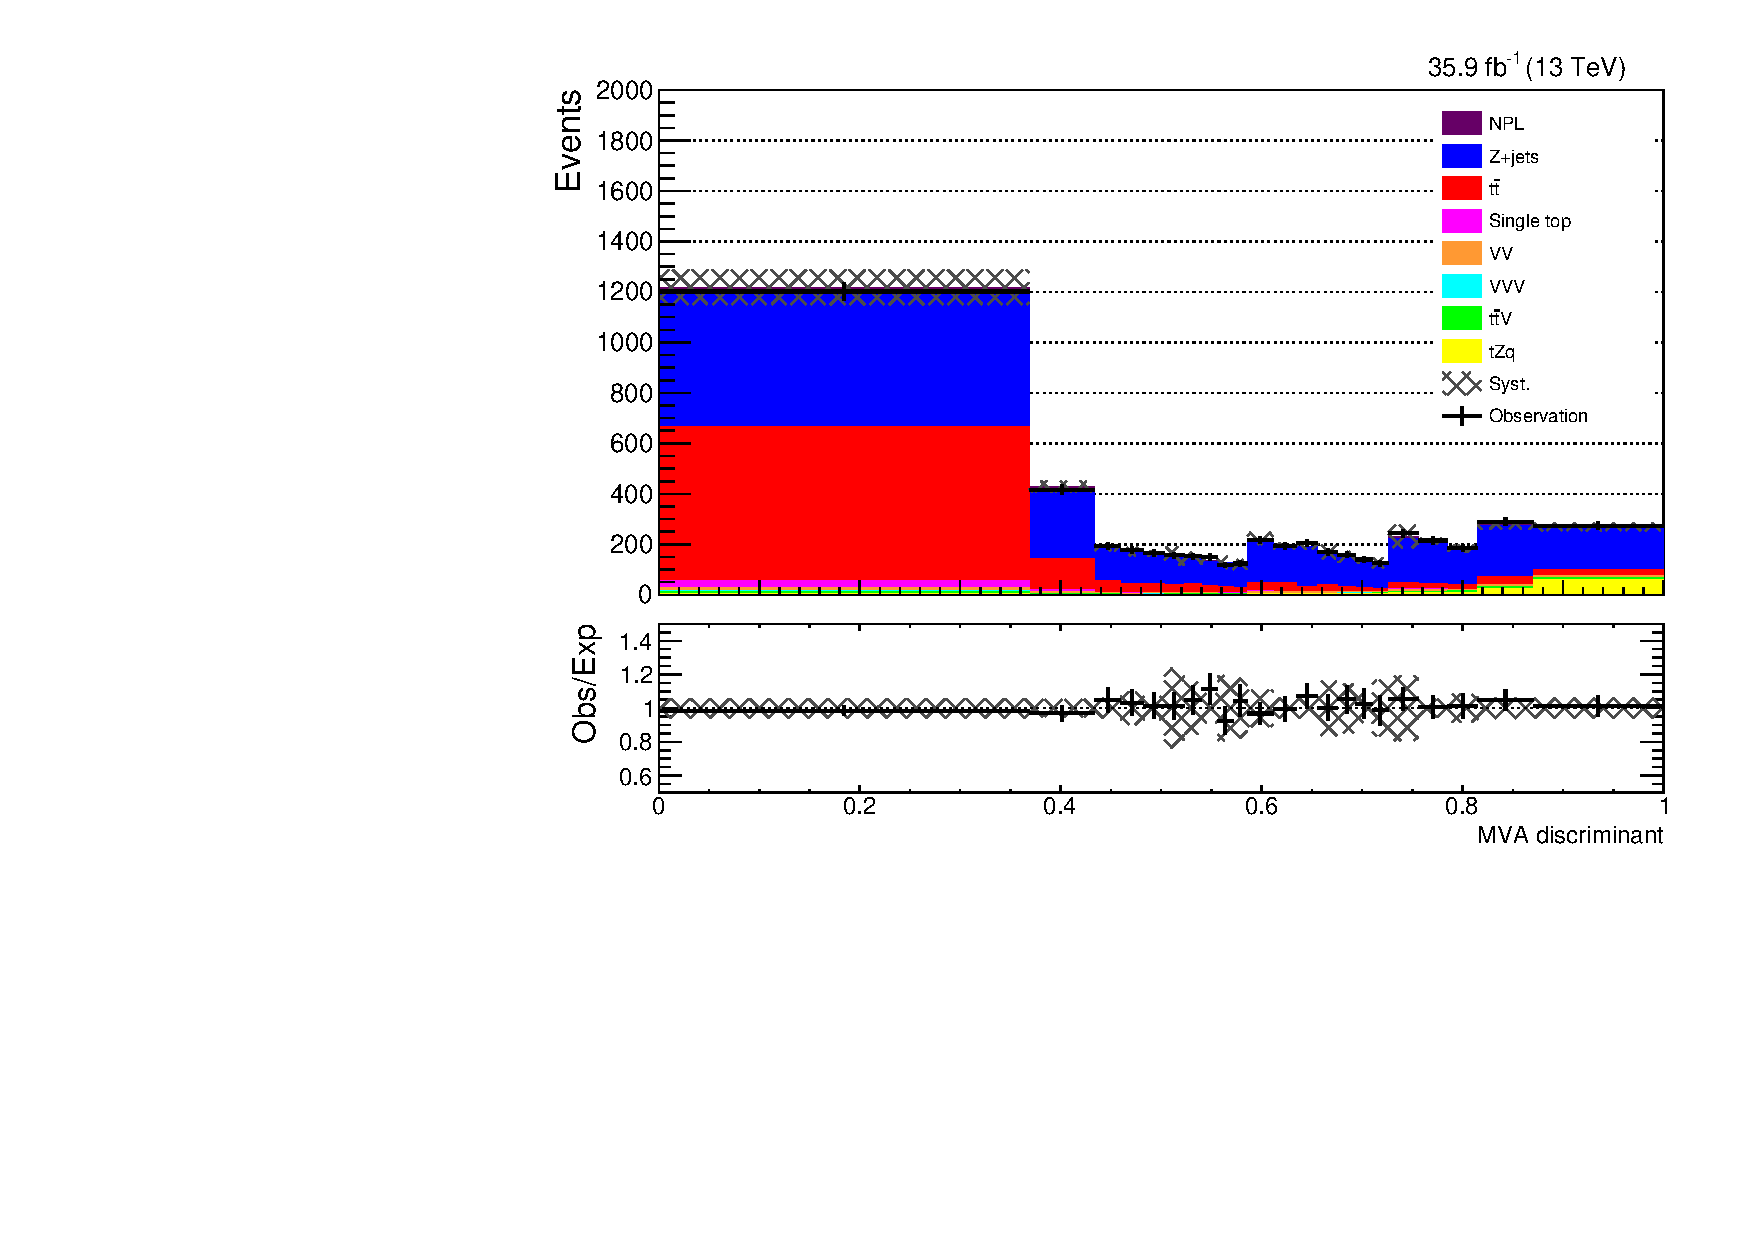
\includegraphics[width=0.78\textwidth]{figs/results/postfit_ee.pdf}
\\
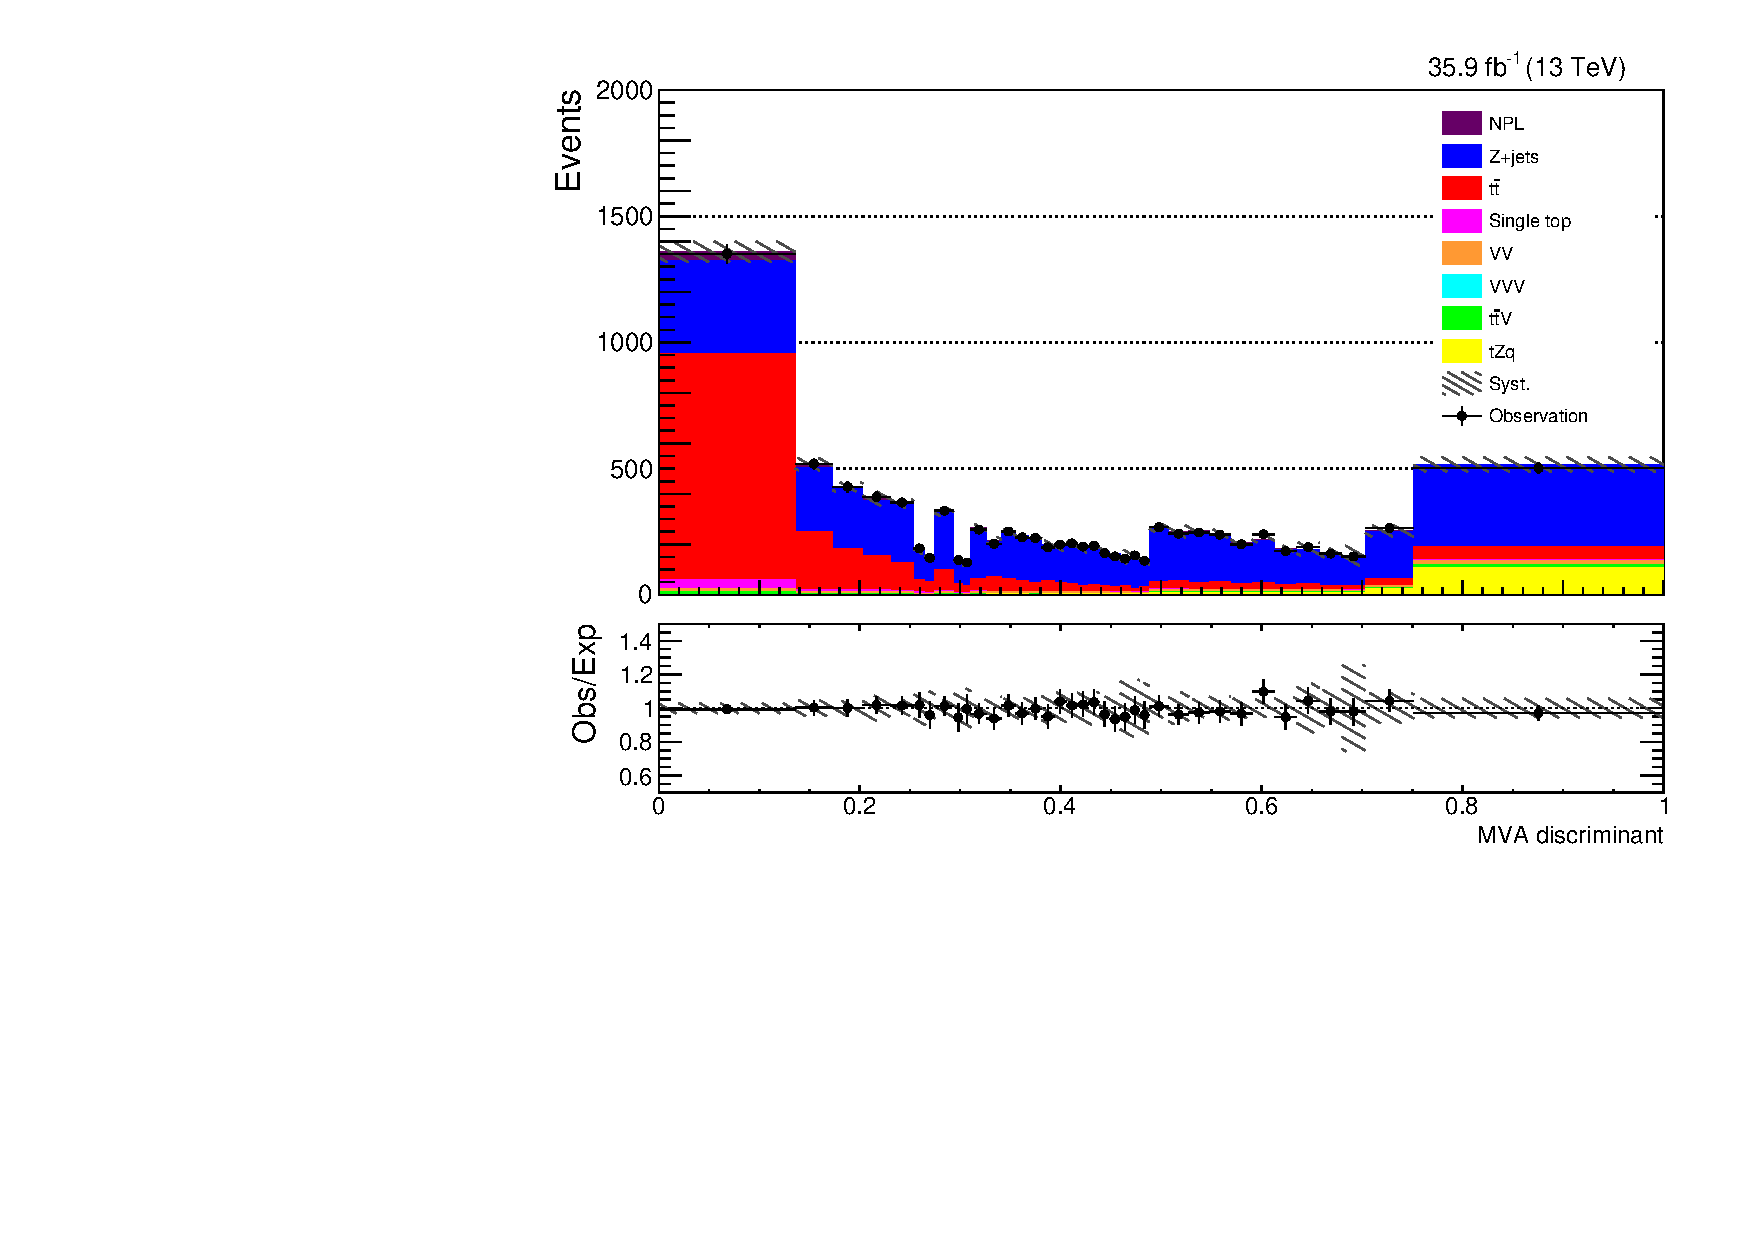
\includegraphics[width=0.78\textwidth]{figs/results/postfit_mumu.pdf}
\caption{
Post-fit distributions of the BDT discriminant for the $ee$ channel (top) and $\mu\mu$ channel (bottom).}
\label{fig:postfitBDT}
\end{figure}

\subsection{Post-fit Impact of the Systematic Uncertainties}\label{sec:uncertainitiesImpact}
Figure~\ref{fig:systematicsPull} illustrates the impact of each of the sources of systematic uncertainty on the signal strength modifier $\mu$ for the $ee$ and $\mu\mu$ channels.
The left-hand side of this plot shows best fit value of the nuisance parameters where the asymmetric error bars are the pre-fit uncertainty divided by the post-fit uncertainty.
The right-hand side illustrates the impact of varying a nuisance parameter to its $\pm \sigma$ post-fit values on the $\mu$.

It can be seen in Figure~\ref{fig:systematicsPull} that despite being constrained in the fit like the majority of the experimental uncertainties, the impact of the PDFs uncertainties on the $\mu$ is similar to those from the constrained theoretical scale uncertainties.
While normalisation of the contributions from the non-prompt lepton and minor background processes are not further constrained in the MLF, they have the smallest impact on the $\mu$.
The nuisance parameters for both the normalisation of the \ttbar and Z+jets background processes are constrained, but are offset from their pre-fit values to varying degrees in both channels.
This implies that ...

\begin{figure}[Htbp]
\begin{center}
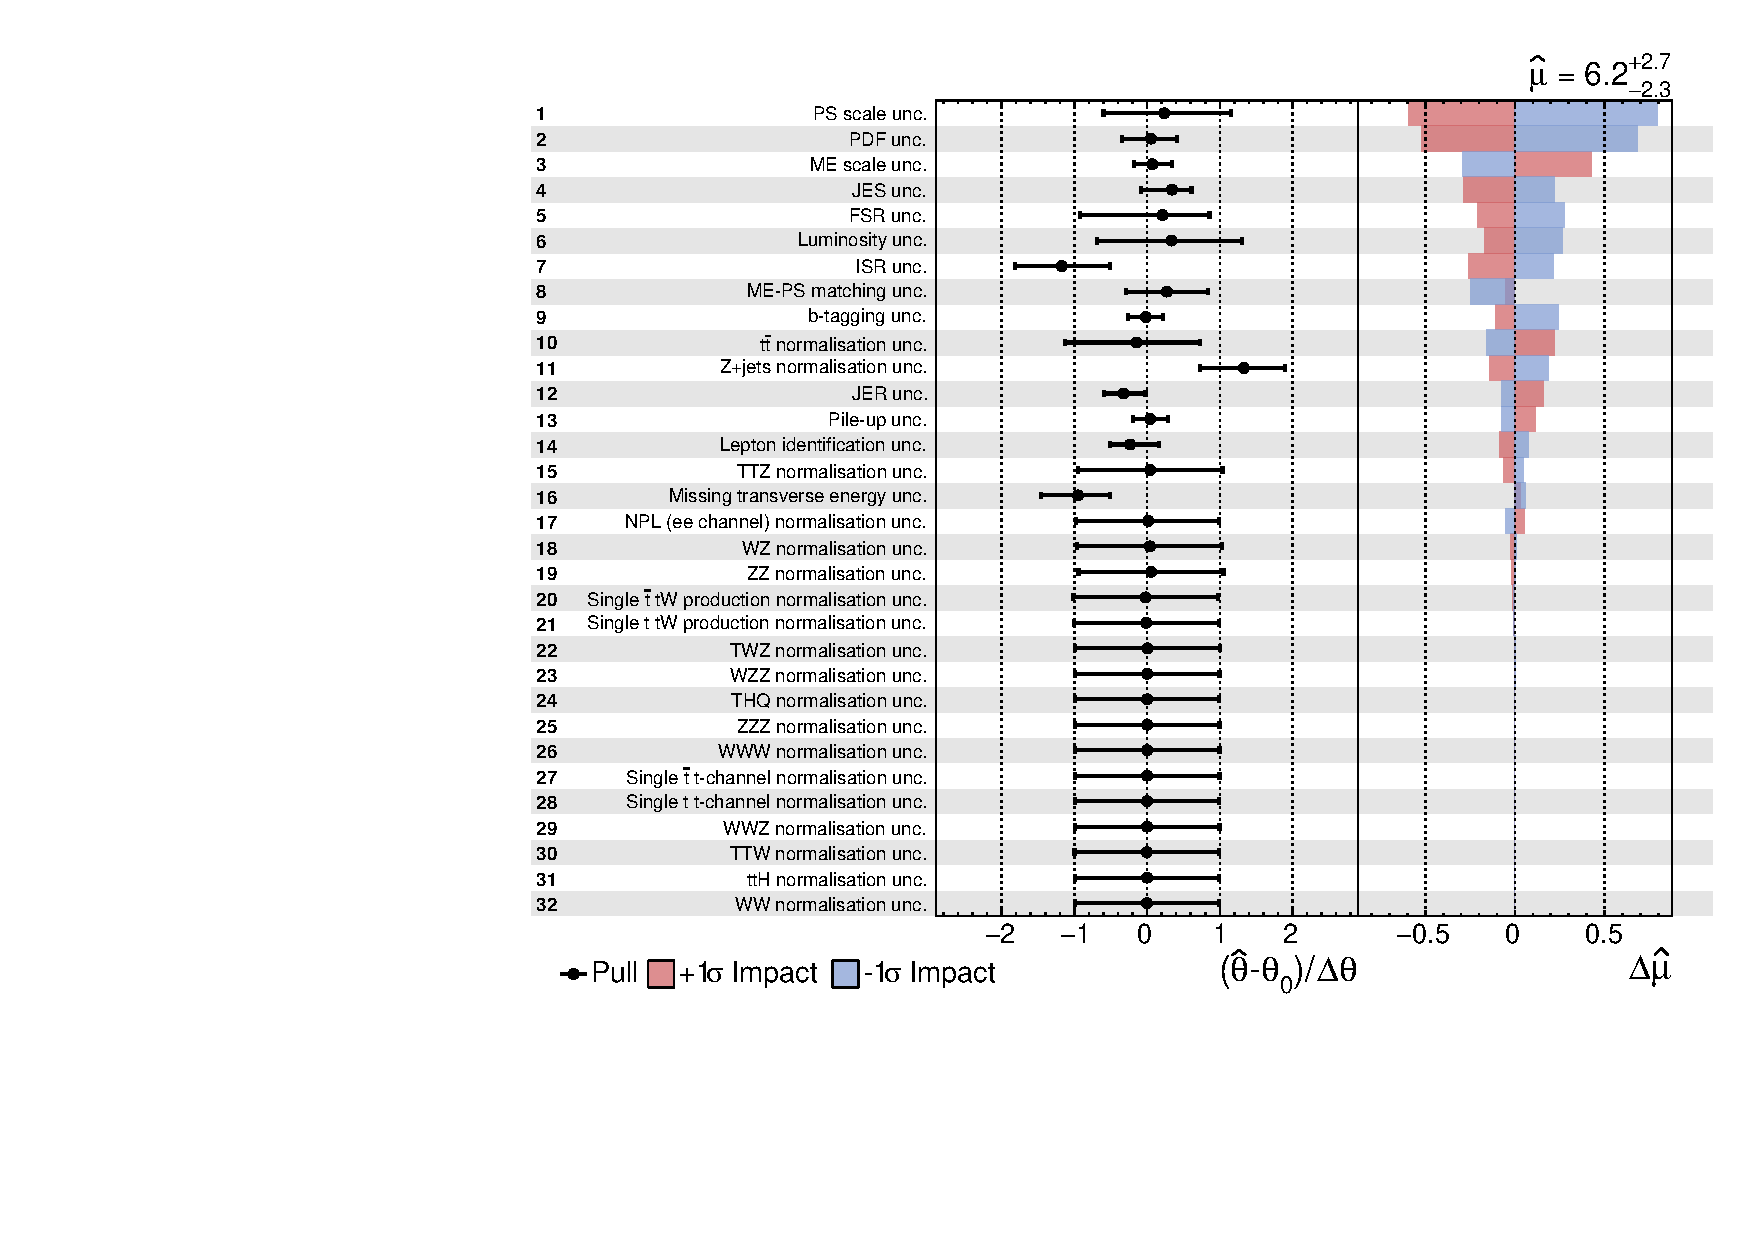
\includegraphics[width=0.97\textwidth]{figs/results/systematicsImpact_ee.pdf}
\\
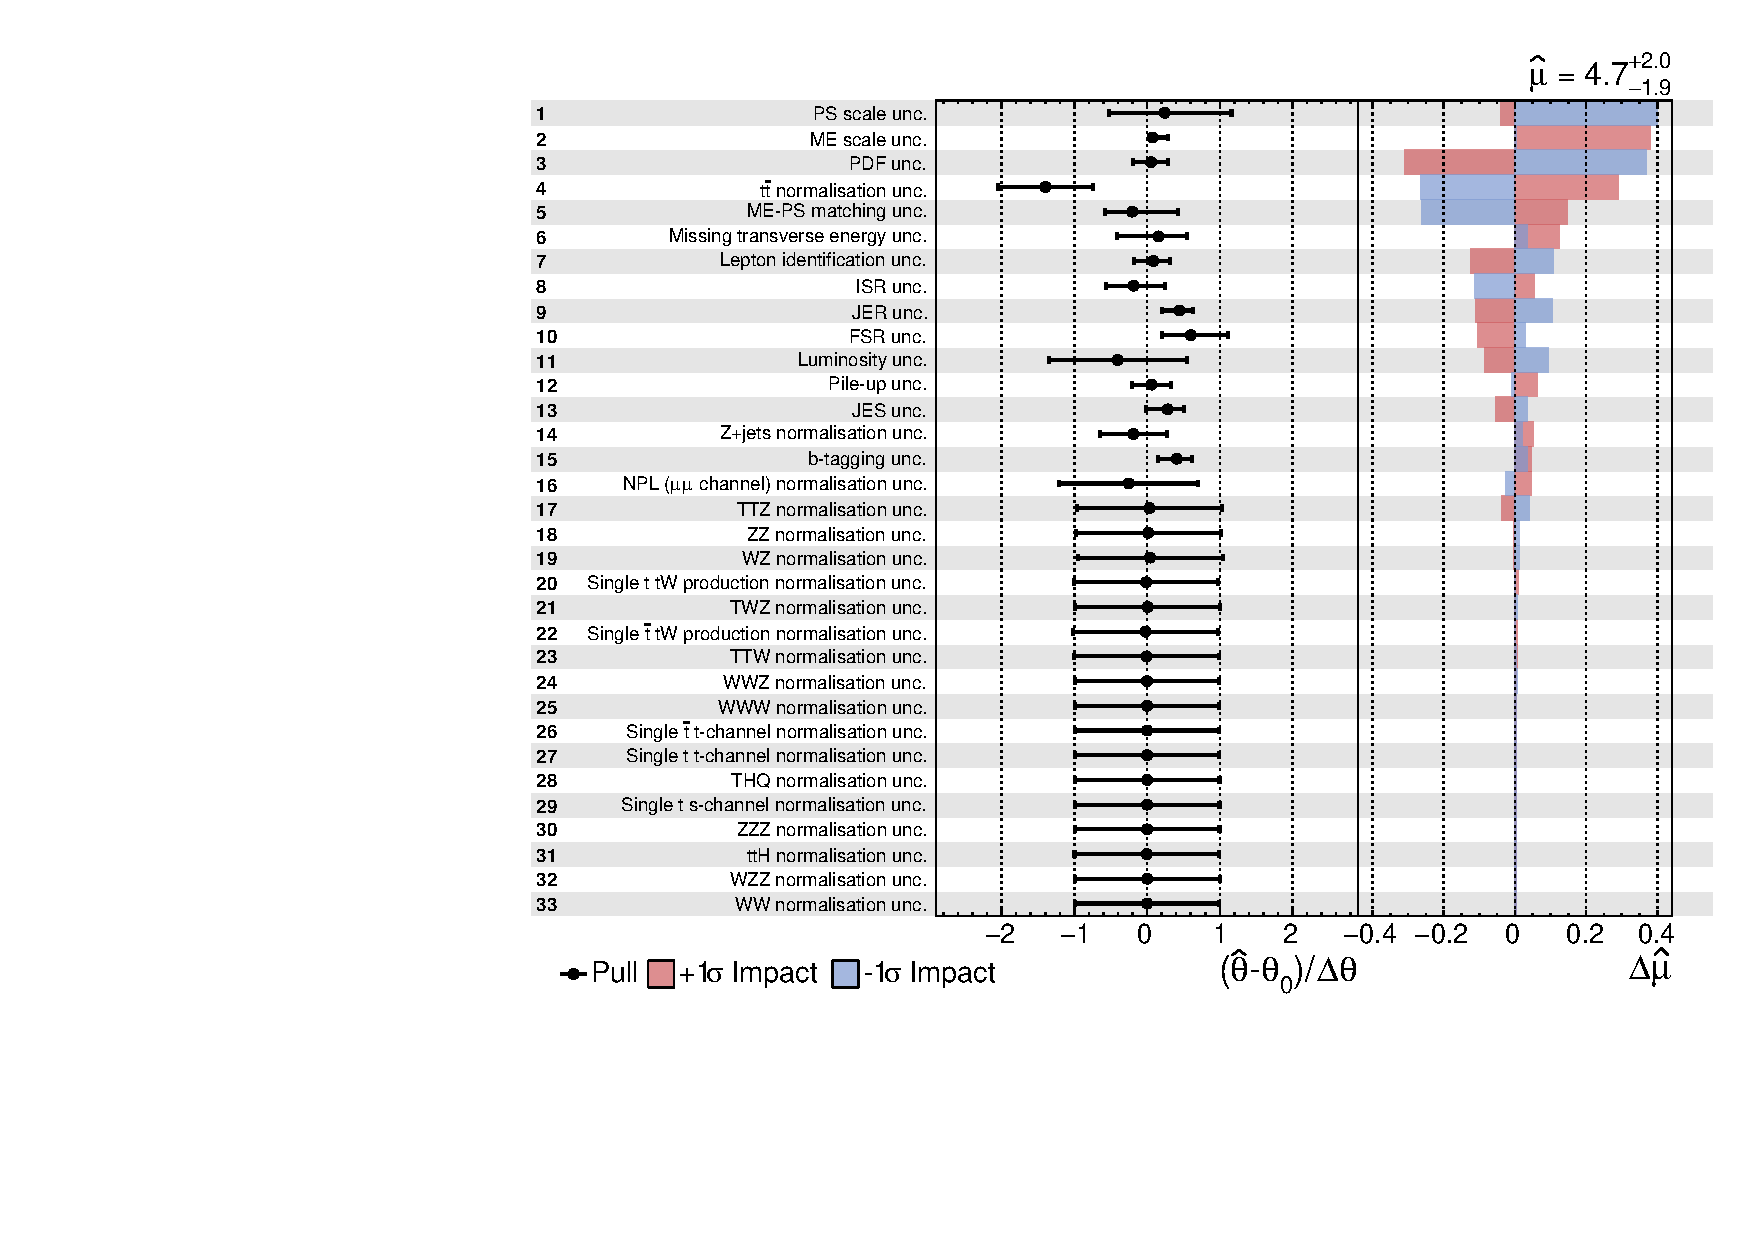
\includegraphics[width=0.97\textwidth]{figs/results/systematicsImpact_mumu.pdf}
\caption{The best fit value and uncertainties of the nuisance parameters are shown on the left-hand side of the plot, where $\widehat{theta}$ and $theta_{0}$ are the post-fit and pre-fit values for a nuisance parameter and $\Delta \theta$ is the pre-fit uncertainty.
The right-hand side of the plot shows the impact that each systematic uncertainty has on the signal strength parameter $\mu$ when varied by $\pm 1 \sigma$.
The top and bottom plots refer to the $ee$ and $\mu\mu$ channels, respectively.}
\label{fig:systematicsPull}
\end{center}
\end{figure}

\section{Discussion of other searches for tZq at the Large Hadron Collider}
The search for the decay of a single top quark produced in association with a Z boson presented in this thesis is the first one that has been made using the dilepton final state at the LHC.

Previously the production of a single top quark in association with a Z boson has been searched for using the trilepton final state at the LHC using proton-proton collision data at $\sqrt{s} = 8 \TeV$ and $\sqrt{s} = 13 \TeV$.
tZq production was initially searched for using the trilepton final state at $\sqrt{s} = 8 \TeV$ by the CMS Collaboration~\cite{Sirunyan:2017kkr}, which made a measurement with an observed significance of $2.9 \sigma$.
The first observation of tZq using the trilepton final state was made by the ATLAS and CMS collaborations at $\sqrt{s} = 13 \TeV$, 

$0.75 \pm 0.28$ ATLAS and $1.45^{0.48}_{-0.42}$ CMS

with observed(expected) significances of 4.2(5.4) and 3.7(3.1) standard deviations, respectively~\cite{Aaboud:2017ylb,Sirunyan:2017nbr}.
In contrast, the expected significance of measuring tZq using the dilepton final state at $\sqrt{s} = 13 \TeV$ was significantly smaller at $0.70\sigma$.

The difference between the sensitivity of measuring tZq using the trilepton and dilepton final states is due to the relative sizes of their background contributions.
The presence of a third lepton in the trilepton final state suppresses the 
In contrast, the requirement for two well-defined promptly produced leptons for the dilepton final state suppresses 
 
While contributions from WZ processes and those involving NPLs form the largest backgrounds for the searches using the trilepton final state, as the 

Both ATLAS+CMS uses CRs to constrain NPLs

Therefore, given that the lack of sufficient statistics is the main factor limiting the significance of the result presented, it is essential to extend this search to include additional data collected by the CMS experiment if tZq is to be observed using the dilepton final state.